% !TeX root = surprises.tex

\chapter%
[הבעיה של 
\L{\normalsize Langford}]%
{הבעיה של 
\L{\Large Langford}}
\label{c.langford}

המתמטיקאי
\L{C. Dudley Langford}
שם לב שבנו סידר קוביות צבעוניות לפי הסדר באיור%
~\ref{f.langford}.
קוביה אחת נמצאת בין שתי הקוביות האדומות, שתי קוביות בין הקוביות הכחולות, ושלוש קוביות בין הקוביות הירוקות.  
\begin{figure}[h]
\begin{center}
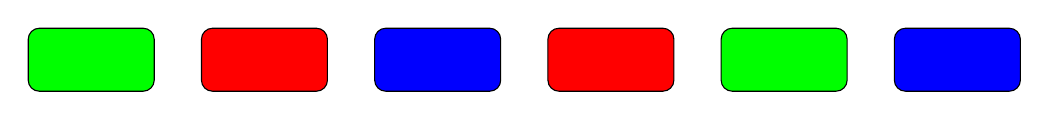
\begin{tikzpicture}
\draw[rounded corners,fill=green] (0,0)  
  rectangle +(1.6cm,.8cm);
\draw[rounded corners,fill=red]   (2.2,0)
  rectangle +(1.6cm,.8cm);
\draw[rounded corners,fill=blue]  (4.4,0)
  rectangle +(1.6cm,.8cm);
\draw[rounded corners,fill=red]   (6.6,0)
  rectangle +(1.6cm,.8cm);
\draw[rounded corners,fill=green] (8.8,0)
  rectangle +(1.6cm,.8cm);
\draw[rounded corners,fill=blue]  (11,0)
  rectangle +(1.6cm,.8cm);
\end{tikzpicture}
\end{center}
\caption{סידור הקוביות לבעיה של \L{Langford}}\label{f.langford}
\end{figure}

\begin{definition}[הבעיה של
\L{Langford} $L(n)$]
נתון שק%
\footnote{\R{
שק
\L{(bag)}
הוא  קבוצה בה איבר יכול להופיע מספר פעמים}.} 
של מספרים
\[
\{1,1,2,2,3,3,\ldots,n,n\}\,,
\]
האם ניתן לסדר אותם כך שלכל
$1\leq i \leq n$, $i$
מספרים נמצאים בין שני המופעים של
$i$?
\end{definition}
מאיור%
~\ref{f.langford}
אנו רואים שעבור 
$n=3$
הפתרון הוא
$312132$.

סעיף%
~\ref{s.langford-covering} 
מנסח מחדש את הבעיה של
\L{Langford}
ביצוג מתמטי שמקל על הפתרון. סעיף%
~\ref{s.langford-theorem}
מאפיין את הערכים 
$n$
עבורם ניתן למצוא פתרון ומביא שתי הוכחות של המשפט. ההוכחה הראשונה פשוטה יחסית ומשתמשת בשיטה של ספירה כפולה: לספור אותו הערך בשתי דרכים שונות ולהשוות את הנוסחאות שמתקבלת. ההוכחה השנייה היא אינדוקציה יפה אבל "הפנקסנות" בהוכחה מחייבת תשומת לב רבה לפרטים. בסעיף%
~\ref{s.langford-four}
נמחשב את הפתרון עבור
$L(4)$.

%%%%%%%%%%%%%%%%%%%%%%%%%%%%%%%%%%%%%%%%%%%%%%

\section{הבעיה של
\L{\normalsize Langford}
כבעיית כיסוי}
\label{s.langford-covering}

ניתן להציג את הבעיה של
\L{Langford}
באמצעות טבלה. עבור
$L(3)$
יש
$6$
עמודות, אחת לכל מקום בסדרה. השורות מציגות את כל האפשרויות למקם את  שני המופעים של אחד המספרים, כלומר, שני המופעים של
$k$
חייבים להיות מוקמים עם 
$k$
עמודות ביניהם. קל לראות שיש ארבעה זוגות של מקומות אפשריים עבור
$1$,
שלושה עבור
$2$
ושניים עבור
$3$:
%)טבלה~%
%\ref{t.lang3:1}(.

%\begin{table}
\[
\begin{array}{|c||c|c|c|c|c|c|}
\hline
&1&2&3&4&5&6\\\hline\hline
1&1&&1&&&\\\hline
2&&1&&1&&\\\hline
3&&&1&&1&\\\hline
4&&&&1&&1\\\hline
5&2&&&2&&\\\hline
6&&2&&&2&\\\hline
7&&&2&&&2\\\hline
8&3&&&&3&\\\hline
9&&3&&&&3\\\hline
\end{array}
\]
%\caption{סידורים אפשריים}\label{t.lang3:1}
%\end{table}


כדי לפתור את הבעיה, עלינו לבחור שורה אחת עבור המופעים של
$1$,
שורה אחת עבור המופעים של
$2$
ושורה אחת עבור המופעים של
$3$,
כך שאם נמקם את השורות אחת מעל לשניה, בכל עמודה יש רק מספר אחד.

שורה
$9$
אינה נחוצה בגלל סימטריה: סדרה המתחילה עם השורה
$9$
זהה לסדרה מתקבלת מהפיכת הסדר של סדרה המתקבלת כאשר מתחילים עם שורה
$8$.
שורה 
$8$
היא היחידה המכילה את המספר
$3$
כך שחובה לבחור אותה, והסדרה המתקבלת היא
$3X  X  X  3X$. 
אי אפשר להשתמש בכל שורה שיש לה מספרים בעמודות
$1$
ו-%
$5$,
כי מותר רק מספר אחד בכל מקום. נסמן את השורות שניתן לבחור ושלא ניתן לבחור כך:
$\not 1,2,\not 3,4,\not 5, \not 6, 7, 8$.

שורה
$7$
היא השורה האפשרית היחידה עבור
$2$
כך שחובה לבחור בה והתוצאה היא
$3X  2X  3{}2$.
נעדכן את רשימת השורות ונקבל:
$\not 1,2,\not 3,\not 4,\not 5, \not 6, 7, 8$.

כעת, השורה היחידה שניתן לבחור היא
$2$
ומתקבל הפתרון
$3{}1{}2{}1{}3{}2$.
\[
\begin{array}{|c||c|c|c|c|c|c|}
\hline
&1&2&3&4&5&6\\\hline\hline
2&&1&&1&&\\\hline
7&&&2&&&2\\\hline
8&3&&&&3&\\\hline
\end{array}
\]
הניתוח הראה שאין פתרון אחר פרט לפתרון הסימטרי שמתקבל אם מלחילים עם שורה
$9$.

\section{
מהם הערכים של
$n$
עבורם ניתן לפתור את בעיית
\L{\normalsize Langford}?}
\label{s.langford-theorem}

\begin{theorem} \label{thm.langford}
ניתן למצוא פתרון ל-%
$L(n)$
אם ורק אם
$n=4k$
או
$n=4k-1$.
\end{theorem}
נוכיח רק שאם 
$n=4k-2$
או
$n=4k-3$
אין פתרון לבעיה. ההוכחה הראשונה מוכיחה שאם יש פתרון ל-%
$L(n)$
אזי 
$n=4k$
או
$n=4k+3$.
ההוכחה השנייה מוכיחה את הפך השלילי: אם
$n=4k+1$
או
$n=4k+2$
אזי אין פתרון ל-%
$L(n)$.

\begin{proof}(1)
אם המופע הראשון של המספר
$k$
נמצא במקום
$i_k$,
המופע השני נמצא במקום
$i_k+k+1$.
למשל, ב-%
3{}1{}2{}1{}3{}2,
הפתרון עבור
$L(3)$,
אם נבחר
$k=2$,
$i_k=3$
ו-%
$i_k+k+1=3+2+1=6$.

$S_n$,
סכום המקומות של כל המספרים, הוא:
\begin{eqn}
S_n&=&\sum_{k=1}^{n}i_k+\sum_{k=1}^{n}(i_k+k+1)\\
& =& 2\sum_{k=1}^{n}i_k+\sum_{k=1}^{n}(k+1)\\
&=& 2\sum_{k=1}^{n}i_k+\frac{n(n+3)}{2}\,.
\end{eqn}
אבל
$S_n$
הוא פשוט
$1+2+3+\cdots+2n$
כך ש:
\[
S_n=\sum_{k=1}^{2n}k = \frac{2n(2n+1)}{2}\,.
\]
נשווה את שני הביטויים עבור
$S_n$
ונקבל:
\begin{eqn}
2\sum_{k=1}^{n}i_k+\frac{n(n+3)}{2} &=& \frac{2n(2n+1)}{2}\\
\sum_{k=1}^{n}i_k &=& \frac{1}{2}\left(\frac{2n(2n+1)}{2} - \frac{n(n+3)}{2}\right) \\
&=& \frac{3n^2-n}{4}\,.
\end{eqn}
הצד השמאלי חייב להיות מספר שלם כי הוא סכום של מספרים שלמים (מיקומים), ולכן, הצד הימני חייב גם הוא להיות מספר שלם. מתי
$3n^2-n$
מתחלק ב-%
$4$?
נפרק את
$3n^2-n$
ונקבל
$n(3n-1)$.

אם
$n$
מתחלק ב-%
$4$,
המכפלה מתחלקת ב-%
$4$.



מתי 
$3n-1$
מתחלק ב-%
$4$?
ניתן לייצג כל מספר שלם
$n$
כ-%
$n=4i+j$
עבור
$j=0,1,2,3$.
אם 
$3n-1$
מתחלק ב-%
$4$,
גם
$3(4i+j)-1 = 12i+3j-1$
מתחלק ב-%
$4$.
ברור ש-%
$12i$
מתחלק ב-%
$4$.
עבור
$j=\{0,1,2,3\}$,
$3j-1=\{-1,2,5,8\}$
מתחלק ב-%
$4$
אם ורק אם
$j=3$,
כלומר,
$n=4i+3$.
\end{proof}

כדי להכיר את העיקרון של ההוכחה השנייה, נבדוק איך פתרון עבור
$n=4$
ייראה. בטבלאות שלהלן המקומות של 
$4$
הם 
$1$
ו-%
$6$
והמקומות של
$2$
הם
$5$
ו-%
$8$.
בשני המקרים, מקום אחד זוגי ומקום אחד אי-זוגי:
\[
\begin{array}{|c|c|c|c|c|c|c|c|}
\hline
1&2&3&4&5&6&7&8\\
\hline\hline
4&1&3&1&2&4&3&2\\\hline
*&&&&&*&&\\\hline
\end{array}
\hspace{3em}
\begin{array}{|c|c|c|c|c|c|c|c|}
\hline
1&2&3&4&5&6&7&8\\
\hline\hline
4&1&3&1&2&4&3&2\\\hline
&&&&*&&&*\\\hline
\end{array}
\]
ניקח מספר
\textbf{זוגי}
$k=2m$. 
מקום המופע הראשון שלו הוא
$i$
ומקום המופע השני שלו הוא
$i+k+1$.
סכום המקומות הוא:
\[
i+(i+k+1)=2i+2m+1=2(i+m)+1\,,
\]
שהוא מספר אי-זוגי. כדי שהסכום של שני מספרים יהיה אי-זוגיים, אחד חייב להיות זוגי ואחד אי-זוגי.

נבדוק עכשיו את מקומות המופעים של המספרים האי-זוגיים. מקומות המופעים של
$1$
הם
$2$
ו-%
$4$,
ומקומות המופעים של
$3$
הם
$3$
ו-%
$7$,
שניהם מספרים אי-זוגיים.
\[
\begin{array}{|c|c|c|c|c|c|c|c|}
\hline
1&2&3&4&5&6&7&8\\
\hline\hline
4&1&3&1&2&4&3&2\\\hline
&*&&*&&&&\\\hline
\end{array}
\hspace{3em}
\begin{array}{|c|c|c|c|c|c|c|c|}
\hline
1&2&3&4&5&6&7&8\\
\hline\hline
4&1&3&1&2&4&3&2\\\hline
&&*&&&&*&\\\hline
\end{array}
\]
ניקח מספר 
\textbf{אי-זוגי},
$k=2m+1$.
סכום המקומות הוא:
\[
i+(i+k+1)=2i+2m+1+1=2(i+m+1)\,,
\]
שהוא מספר זוגי. סכום של שני מספרים הוא זוגי אם ורק אם שניהם זוגיים או שניהם אי-זוגיים.

רשימת המקומות של המספרים בסדרה,
$1,2,\ldots,2n-1,2n$,
מכילה מספר שווה של מקומות זוגיים ומקומות אי-זוגיים. כאשר מציבים את שני המופעים של מספר בסדרה, הם "תופסים" שני מקומות. כאשר מסיימים להציב את כל המספרים בפתרון, חייבים להיות מספר שווה של מקומות זוגיים ואי-זוגיים "שנתפסו". נגדיר את 
\textbf{הזוגיות}
כהפרש בין מספר המקומות הזוגיים שנתפסו לבין מספר המקומות האי-זוגיים שנתפסו. תחילה הזוגיות היא אפס, ואם יש פתרון זוגיות שלו גם כן אפס.


כאשר ממקמים את שני המופעים של מספר זוגי, הם תופסים מקום אחד זוגי (מסומן 
$+1$)
ומקום אחר אי-זוגי (מסומן 
$-1$),
והזוגיות לא משתנה:
\[
\begin{array}{|c|c|c|c|c|c|c|c|}
\hline
1&2&3&4&5&6&7&8\\
\hline\hline
4&1&3&1&2&4&3&2\\\hline
-1&&&&&+1&&\\\hline
\end{array}
\hspace{3em}
\begin{array}{|c|c|c|c|c|c|c|c|}
\hline
1&2&3&4&5&6&7&8\\
\hline\hline
4&1&3&1&2&4&3&2\\\hline
&&&&-1&&&+1\\\hline
\end{array}
\]
כאשר ממקמים את שני המופעים של מספר אי-זוגי, הזוגיות משתנה ב-%
$+2$
או 
$-2$,
ולכן עלינו לייחס את הזוג הזה עם זוג מופעים של מספר אי-זוגי אחר כדי לאפס את שנוי בזוגיות:
\[
\begin{array}{|c|c|c|c|c|c|c|c|}
\hline
1&2&3&4&5&6&7&8\\
\hline\hline
4&1&3&1&2&4&3&2\\\hline
&+1&&+1&&&&\\\hline
\end{array}
\hspace{3em}
\begin{array}{|c|c|c|c|c|c|c|c|}
\hline
1&2&3&4&5&6&7&8\\
\hline\hline
4&1&3&1&2&4&3&2\\\hline
&&-1&&&&-1&\\\hline
\end{array}
\]
הראנו שיש פתרון לבעיית
\L{Langford}
אם ורק אם יש מספר זוגי של מספרים אי-זוגיים ב-%
$\{1,\ldots,n\}$!
המשפט טוען שזה נכון אם 
$n=4k$
או
$n=4k\!-\!1$
והמשפט לא-נכון אם
$n=4k\!-\!2$
או
$n=4k\!-\!3$.

\begin{proof}(2)
ההוכחה באינדוקציה. קיימות ארבע טענות בסיס:
\begin{itemize}
\item $n=4k-3=1$.
ב-%
$\{1\}$
יש מספר אי-זוגי של אי-זוגיים ואין פתרון.
\item $n=4k-2=2$.
ב-%
$\{1,2\}$
יש מספר אי-זוגי של אי-זוגיים ואין פתרון.
\item $n=4k-1=3$.
ב-%
$\{1,2,3\}$
יש מספר זוגי של אי-זוגיים וראינו שיש פתרון.
\item $n=4k-0=4$.
ב-%
$\{1,2,3,4\}$
יש מספר זוגי של אי-זוגיים ופתרון נמצא בסעיף%
~\ref{s.langford-four}.
\end{itemize}
הנחת האינדוקציה היא שהמשפט נכון עבור 
$\}\{1,\ldots,4k-j\}$,
$k\geq 1, 0\leq j\leq 3$,
ונוכיח שהמשפט נכון עבור
$n=4(k+1)-j$.
\begin{itemize}
\item
נוסיף
$4k+1=4(k+1)-3$
ל-%
$\{1,\ldots,4k\}$. 
לפי הנחת האינדוקציה עבור
$4k=4k-0$ 
קיים מספר זוגי של מספרים אי-זוגיים.
$4(k+1)-3$
אי-זוגי ולכן עכשיו יש מספר אי-זוגי של מספרים אי-זוגיים ואין פתרון.
\item 
נוסיף
$4k+2=4(k+1)-2$
ל-%
$\{1,\ldots,4k+1\}$.
לפי הנחת האינדוקציה עבור
$4k+1=4(k+1)-3$
קיים מספר אי-זוגי של מספרים אי-זוגיים.
$4(k+1)-2$
זוגי ולכן עכשיו עדיין יש מספר אי-זוגי של מספרים אי-זוגיים ואין פתרון.
\item 
נוסיף
$4k+3=4(k+1)-1$
ל-%
$\{1,\ldots,4k+2\}$.
לפי הנחת האינדוקציה עבור
$4k+2=4(k+1)-2$
קיים מספר אי-זוגי של מספרים אי-זוגיים.
$4(k+1)-1$
אי-זוגי ולכן עכשיו יש מספר זוגי של מספרים אי-זוגיים וסביר שיש פתרון.
\item 
נוסיף
$4k+4=4(k+1)-0$
ל-%
$\{1,2,\ldots,4k+3\}$.
לפי הנחת האינדוקציה עבור
$4k+3=4(k+1)-1$
קיים מספר זוגי של מספרים אי-זוגיים.
$4(k+1)-0$
זוגי ולכן עכשיו יש מספר זוגי של מספרים אי-זוגיים וסביר שיש פתרון.
\end{itemize}
\end{proof}

%%%%%%%%%%%% Solution for L(4) %%%%%%%%%%%%%%%%%%

\newpage

\section{פתרון עבור
$L(4)$}\label{s.langford-four}

הנה הטבלה עבור
$L(4)$.
אל תמשיך לקרוא לפני שתנסה בעצמך למצוא פתרון.
\begin{center}
\selectlanguage{english}
\addtolength{\tabcolsep}{4pt}
\begin{tabular}{|c||c|c|c|c|c|c|c|c|}
\hline
&1&2&3&4&5&6&7&8\\\hline\hline
1&1&&1&&&&&\\\hline
2&&1&&1&&&&\\\hline
3&&&1&&1&&&\\\hline
4&&&&1&&1&&\\\hline
5&&&&&1&&1&\\\hline
6&&&&&&1&&1\\\hline
7&2&&&2&&&&\\\hline
8&&2&&&2&&&\\\hline
9&&&2&&&2&&\\\hline
10&&&&2&&&2&\\\hline
11&&&&&2&&&2\\\hline
12&3&&&&3&&&\\\hline
13&&3&&&&3&&\\\hline
14&&&3&&&&3&\\\hline
15&&&&3&&&&3\\\hline
16&4&&&&&4&&\\\hline
17&&4&&&&&4&\\\hline
18&&&4&&&&&4\\\hline
\end{tabular}
\end{center}
לפי סמטריה ניתן להתעלם משורה
\L{18}.

\noindent 
בחר שורה
\L{16}
והסדרה היא
\L{4XXXX4XX}.
כל שורה עם מספר במקום
$1$
או במקום
$6$
כבר לא יכול להיות חלק מהפתרון.

$\not\! 1,2,3,\not\! 4,5,\not\! 6,\not\! 7,8,\not\! 9,10,11,\not\!\! 12,\not\!\! 13,14,15,16,\not\!\! 17$

\noindent
בחר שורה
\L{14}
והסדרה היא
\L{4X3XX43X}.

$\not\! 1,2,\not\! 3,\not\! 4,\not\! 5,\not\! 6,\not\! 7,8,\not\! 9,\not\!\! 10,11,\not\!\! 12,\not\!\! 13,14, \not\!\! 15,16,\not\!\! 17$

\noindent
בחר שורה
\L{8}
והסדרה היא
\L{423X243X}.

$\not\! 1,\not\! 2,\not\! 3,\not\! 4,\not\! 5,\not\! 6,\not\! 7,8,\not\! 9,\not\!\! 10,\not\!\! 11,\not\!\! 12,\not\!\! 13,14, \not\!\! 15,16,\not\!\! 17$

\noindent
לא נשארו מקומות עבור הספרה $1$ ולכן עלינו לחזור אחורה.

\smallskip

\noindent 
במקום שורה $8$ בחר שורה $11$ והסדרה היא
\L{4X3X2432}.


$\not\! 1,2,\not\! 3,\not\! 4,\not\! 5,\not\! 6,\not\! 7,\not\! 8,\not\! 9,\not\!\! 10,11,\not\!\! 12,\not\!\! 13,14, \not\!\! 15,16,\not\!\! 17$

\noindent
בחר שורה
\L{2}
ומצאנו פתרון
\L{41312432}.

\smallskip

\noindent
נחזור אחורה ונחפש פתרון אחר.

\smallskip

\noindent
במקום שורה
\L{14}
בחר שורה
\L{15}
והסדרה היא
\L{4XX3X4X3}.

$\not\! 1,\not\! 2,3,\not\! 4,5,\not\! 6,\not\! 7,8,\not\! 9,\not\!\! 10,\not\!\! 11,\not\!\! 12,\not\!\! 13,\not\!\! 14,15,16,\not\!\! 17$

\noindent 
בחר בשורה 8 והסדרה היא
42X324X3.

$\not\! 1,\not\! 2,\not\! 3,\not\! 4,\not\! 5,\not\! 6,\not\! 7,8,\not\! 9,\not\!\! 10,\not\!\! 11,\not\!\! 12,\not\!\! 13,\not\!\! 14,15,16,\not\!\! 17$

לא נשארו מקומות עבור הספרה $1$ ולכן עלינו לחזור אחורה.

\smallskip

\noindent
במקום שורה
\L{16}
בחר שורה
\L{17}
והסדרה היא
\L{X4XXXX4X}.

$1,\not\! 2,3,4,\not\! 5,6,7,\not\! 8,9,\not\!\! 10,11,12,\not\!\! 13,\not\!\! 14,15,\not\!\! 16,17$

\noindent 
בחר שורה
\L{15}
והסדרה היא
\L{X4X3XX43}.

$1,\not\! 2,3,\not\! 4,\not\! 5,\not\! 6,\not\! 7,\not\! 8,9,\not\!\! 10,\not\!\! 11,\not\!\! 12,\not\!\! 13,\not\!\! 14,15,\not\!\! 16,17$

\noindent 
חייבים לבחור שורה
\L{9}
והסדרה היא
\L{X423X243}.

$1,\not\! 2,\not\! 3,\not\! 4,\not\! 5,\not\! 6,\not\! 7,\not\! 8,9,\not\!\! 10,\not\!\! 11,\not\!\! 12,\not\!\! 13,\not\!\! 14,15,\not\!\! 16,17$

\noindent
לא נשארו מקומות עבור הספרה $1$ ולכן עלינו לחזור אחורה פעם אחת אחרונה.
%$1,\not\! 2,3,4,\not\! 5,6,7,\not\! 8,9,\not\! 10,11,12,\not\! 13,\not\! 14,15,\not\! 16,17$

\smallskip

\noindent
במקום שורה
\L{15}
בחר שורה
\L{12}
והסדרה היא
\L{34XX3X4}.

$\not\! 1,\not\! 2,\not\! 3,\not\! 4,\not\! 5,\not\! 6,\not\! 7,\not\! 8,9,\not\!\! 10,\not\!\! 11,12,\not\!\! 13,\not\!\! 14,\not\!\! 15,\not\!\! 16,17$

\noindent
שוב, לא נשארו מקומות עבור הספרה $1$.

\medskip

\noindent 
לכן הפתרון היחיד הוא
\L{41312432}.

\subsection*{מה ההפתעה?}

מקור ההשראה למשפט מתמטי יכול להיות מפתיע.
\L{Langford}
שם לב לתבנית בבלוקים הצבעוניים של בנו וזה הביא אותו למפשט%
~\ref{thm.langford}.
רצוי שסטודנטים ייחפו להוכחות שונות למשפט אחד.

\subsection*{מקורות}
פרק זה מבוסס על
\cite{miller}.
\cite{davies}
מראה איך למצוא פתרון עבור
$n=4k$
ו-%
$n=4k+3$.
